\documentclass[letterpaper,12pt]{article}
\usepackage{ifthen}
\usepackage{times}
\usepackage{amsmath}
\usepackage{amssymb}
\usepackage{helvet}
\usepackage{courier}
\usepackage{fancyheadings}
\usepackage{hyperref}
\usepackage{comment}
\pagestyle{fancy}
\usepackage{pmc}
\usepackage{graphicx}
\setlength\textwidth{6.5in}
\setlength\textheight{8.5in}

%%%%%%%%%%%%%%%%%%%%%%%%%%%%%%%%%%%%%%%%%%%%%%%%%%%%%%%%%%%%%%%%%%%%%%%%%%%%%%%%%%
% Special for e-unibus doc commands

\newcommand{\ForLater}{
\begin{center}
{\bf NOT FOR CURRENT VERSION}
\end{center}
}
\newcommand{\TBC}{\framebox{\textbf{TO BE COMPLETED}}}
\newcommand{\DISCUSS}{\Ovalbox {\bf \textcolor{red}{FOR DISCUSSION}}}
\newcommand{\Input}{\framebox{\textsf{in}}}
\newcommand{\Output}{\framebox{\textsf{out}}}
\newcommand{\debug}[1]{\textbf{debug start} #1 \textbf{debug finish}}
\newcommand{\inx}[1]{\emph{#1}}
\newtheorem{notation}{Notation}
\newtheorem{definition}{Definition}
\newtheorem{problem_statement}{Problem Statement}
\newtheorem{invariant}{Invariant}
\newtheorem{assumption}{Assumption}
\newtheorem{resource_string}{Resource String}
\newtheorem{testcase}{Test Case}
\newtheorem{note}{Note}
\newtheorem{specification}{Specification}
\newtheorem{caution}{Caution}
\newtheorem{prereq}{Pre-requisite}
\newtheorem{action}{Action}
\newtheorem{query}{Query}
\newcommand{\beq}{\begin{equation}} %% new, no conflict
\newcommand{\eeq}{\end{equation}} %% new, no conflict
\newcommand{\be}{\begin{enumerate}}
\newcommand{\ee}{\end{enumerate}}
\newcommand{\bi}{\begin{itemize}}
\newcommand{\ei}{\end{itemize}}
\newcommand{\bv}{\begin{verbatim}}
\newcommand{\ev}{\end{verbatim}}
\newcommand{\bd}{\begin{description}}
\newcommand{\ed}{\end{description}}
\newcommand{\bpre}{\begin{prereq}}
\newcommand{\epre}{\end{prereq}}
\newcommand{\bact}{\begin{action}}
\newcommand{\eact}{\end{action}}
\newcommand{\bs}{\begin{specification}}
\newcommand{\es}{\end{specification}}
\newcommand{\btc}{\begin{testcase}}
\newcommand{\etc}{\end{testcase}}
\newcommand{\bc}{\begin{caution}}
\newcommand{\ec}{\end{caution}}
\newcommand{\la}{\leftarrow}
\newcommand{\IpArgs}{\subsection{Input Arguments}}
\newcommand{\PreReqs}{\subsection{Pre-requisities}}
\newcommand{\Actions}{\subsection{Actions}}
\newcommand{\Coverage}{{\bf To test coverage.}}

%%%%%%%%%%%%%%%%%%%%%%%%%%%%%%%%%%%%%%%%%%%%%%%%%%%%%%%%%%%%%%%%%%%%%%%%%%%


\newtheorem{theorem}{Theorem}[section]
\newtheorem{lemma}[theorem]{Lemma}
\newtheorem{proposition}[theorem]{Proposition}
\newtheorem{corollary}[theorem]{Corollary}

\newenvironment{proof}[1][Proof]{\begin{trivlist}
\item[\hskip \labelsep {\bfseries #1}]}{\end{trivlist}}
\newenvironment{intuition}[1][Intuition]{\begin{trivlist}
\item[\hskip \labelsep {\bfseries #1}]}{\end{trivlist}}
%% \newenvironment{definition}[1][Definition]{\begin{trivlist}
%% \item[\hskip \labelsep {\bfseries #1}]}{\end{trivlist}}
\newenvironment{example}[1][Example]{\begin{trivlist}
\item[\hskip \labelsep {\bfseries #1}]}{\end{trivlist}}
\newenvironment{remark}[1][Remark]{\begin{trivlist}
\item[\hskip \labelsep {\bfseries #1}]}{\end{trivlist}}

\newcommand{\qed}{\nobreak \ifvmode \relax \else
      \ifdim\lastskip<1.5em \hskip-\lastskip
      \hskip1.5em plus0em minus0.5em \fi \nobreak
      \vrule height0.75em width0.5em depth0.25em\fi}

%%%%%%%%%%%%%%%%%%%%%%%%%%%%%%%%%%%%%%%%%%%%%%%%%%%%%%%%%%%%%%%%%
% \newcommand{\Alogon}{\mbox{\fontfamily{ptm}\selectfont {\large \selectfont A} \hspace{-1.2ex} {\large \selectfont L} \hspace{-2.3ex} \raisebox{0.45ex}{ {\footnotesize \selectfont O} } \hspace{-1.80ex} {\large \selectfont G} \hspace{-1.80ex} \raisebox{-0.33ex}{ {\large \selectfont O} } \hspace{-1.8ex} {\large \selectfont N}}}



\newcommand{\beq}{\begin{equation}} %% new, no conflict
\newcommand{\eeq}{\end{equation}} %% new, no conflict
\newcommand{\bdm}{\begin{displaymath}} %% new, no conflict
\newcommand{\edm}{\end{displaymath}} %% new, no conflict
% \newcommand{\reals}{{\rm I\! R}} %% new, no conflict
\newcommand{\reals}{\cal{R}} %% new, no conflict
% \newcommand{\mymean}[1]{\mu({#1})}
\newcommand{\bb}[1]{\mathbf{#1}}
\newboolean{longform}
\setboolean{longform}{false}
\newboolean{blogpost}
\setboolean{blogpost}{true}
%% Another option is \usepackage{comment}
%% \includecomment(answer} or excludecomment{answer} % then
%% \begin{answer} ... \end{answer}


%% From https://math.berkeley.edu/~gbergman/misc/hacks/langl_rangl.html
\newcommand{\langl}{\begin{picture}(4.5,7)
\put(1.1,2.5){\rotatebox{60}{\line(1,0){5.5}}}
\put(1.1,2.5){\rotatebox{300}{\line(1,0){5.5}}}
\end{picture}}

\newcommand{\rangl}{\begin{picture}(4.5,7)
\put(.9,2.5){\rotatebox{120}{\line(1,0){5.5}}}
\put(.9,2.5){\rotatebox{240}{\line(1,0){5.5}}}
\end{picture}}

\newcommand{\mymean}[1]{\ensuremath{\langl{#1}\rangl}} %% new, no conflict

\begin{document}
\title{Analysis of Binary Outcome A/B Tests - New Metrics}
\author{Ramesh Subramonian, Ranjeet Tate, Michael Shire, Abhi Singh}
\maketitle
\thispagestyle{fancy}
\lhead{}
\chead{}
\rhead{}
\lfoot{}
% \cfoot{{\small NerdWallet Engineering }}
% \rfoot{{\small \thepage}}

As a user (Product Manager, Analyst, HiPPO) of AB tests or a
designer/builder of AB tests and systems: Do you
\bi
\item have a nagging
feeling that though A was statistically better than B, the
difference wasn't large enough to be {\em important}?
\item have
  doubts about the {\em business impact} of the test outcome?
  \item want to
set a single-valued business or revenue goal (e.g. 10\% better) and have a {\em definite recommendation}
made to you instead of dealing with ``we are 90\% confident that A is
11.1\% better than B''?
\item feel overwhelmed by the {\em ``test
  everything''} approach becoming increasingly prevalent in Tech?
  \ei
  If you
answered yes to any of these questions, then read this blog.

First, we need to go beyond asking simply whether ``A is better than
B'' to asking whether ``the difference between A and B
is important enough to be actionable''. Consider an example: The Optimizely
book on A/B testing describes a test comparing a page
with a static ad to one with a video\footnote{``Fail Fast and Learn'',
  pg. 79, {\em A/B Testing}, Dan Siroker and Pete Koomen, Wiley
  (2013)}. The variant with the video was better in terms of both
click-through and conversion rates, but the costs of producing the
video and displaying it were deemed ``too high'' to launch the video
version at scale. So in addition to being statistically significant,
the difference has to be {\em important} enough to recommend
proceeding\footnote{See
  \url{http://shopperscientist.com/archive/views/28may95.html} and
  \url{http://www.med.uottawa.ca/sim/data/Statistical_significance_importance_e.htm}
  for lengthier discussions.}.

Second, this difference has to be evaluated not in terms of the usual
probability but in terms of a revenue or business metric, which
may not be simply related to the measured probability. E.g., in
order to trigger a recommendation, do we want the {\em difference}
between success probabilities to exceed \(0.1\)
---i.e. \(p_A-p_B>0.1\)--- or do we want the success probability to
{\em lift} by 20\% ---i.e. \(p_A > 1.2*p_B\)? Different metrics will
lead to different outcomes. If \(p_B\) happens to be \(0.5\), even
though \(p_A=0.6\) has the same value for both a difference of
\(0.1\) and a lift of \(20\%\), the confidence levels associated with
the two propositions can be quite different.\footnote{Note that the
  choice of comparison metric is an issue that arises {\em only} when
  we want to quantify the comparison. If we were only interested in
  {\em whether} \(A\) is better than \(B\), then any metric (as long
  as it is monotonic in \(p_A\) and \(p_B\)) would do. The choice of
  metric becomes important when we are interested not just in whether
  \(A\) is better than \(B\), but in addition, {\em by how much}.}

Third, decision makers do not want to deal with statements about
``confidence levels in the difference''. The {\em goal of our analysis
  is to provide the test owner with a definite recommendation about
  choosing \(A\) or \(B\)}\footnote{Paraphrasing from Klugman {\em et
    al} ``Loss Models'', 2nd Ed. Wiley (2004), pg. 419: ``...the
  process must end with a winner. While qualifications, caveats
  etc. are often necessary, a commitment is required.'' on the part of the analyst.} based on a
single ``acceptance value'' for a pre-selected business metric.

As a collateral benefit, you may find that the requirement of
calculating a minimum business gain {\em before} starting a test will
magically reduce the number of tests, culling out the more frivolous
ones.

We will illustrate our approach to the first three issues by analysing
the data for binary outcome A/B tests, which we briefly describe.
In a
{\em binary} experiment, each trial has only two possible outcomes, a
{\em success} (1) or a {\em failure} (0).  A population being
experimented on has a ``true'' or intrinsic probability of success \(p\) which is
to be inferred from the results of the test.
In an A/B test there are two populations or branches, each of which is
exposed to a different treatment. The populations have intrinsic success
probabilities \(p_A\) and \(p_B\). After a period of time
(pre-determined by ``power'' calculations or otherwise), the
experiment will yield a count of the trials and successes in each
branch, \((n_A, m_A)\) and \((n_B, m_B)\). From this data we infer a
function that represents the likelihood of \((p_A,p_B)\).

We've taken a Bayesian approach since it turns out to be much better
suited for general metrics. We use the data from the experiment to
construct the posterior probability distribution (or {\em likelihood}) of \((p_A, p_B)\). Fig.~\ref{fig:likelihood} is the two dimensional space of intrinsic probabilities \(\{(p_A,p_B)\}\),
\begin{figure}[ht!]
\centering
\includegraphics[width=90mm]{../presentations/_2_Dimensional_Probability_Space_pA_pB1}
\caption{Contour Plot of the Likelihood of \((p_A, p_B)\) for \((n_A,
  m_A, n_B, m_B) = (12,10,12,7)\). The contours correspond to points of equal likelihood. The insides of high-value contour
  lines represent regions of high likelihood, with
the peak at \((10/12, 7/12)\). \label{fig:likelihood}}
\end{figure}
on which we've shown a contour plot of the likelihood function, see the caption for additional explanation.

The next issue is that of finding a metric which reflects a business interest. Consider a Binary A/B
test in which the probability being measured is the {\em page
  transition probability} \(p\): that of moving to any other page
on the website as opposed to leaving the website or otherwise ending
the session. The business impact is in fact {\em not} proportional to an
increase in the page transition probability. We
know that on average revenue is proportional to clicks, conversions or other
monetizing actions, and that the number of such actions is proportional to 
the number of opportunties to act, which in turn is proportional to
the pages visited on the website. How is the number of page visits
\(PV\) related to the page transition probability \(p\)? Some
thought shows that the average number of pages visited per
user-session is
\beq\label{eq:page_views}
PV= p + p^2 + p^3 + ...= \frac{p}{1-p}
\eeq
which is simply the {\em odds ratio}
corresponding to the probability\footnote{More on this in a separate blog.}!

The same metric also occurs (surprisingly) in the context of loans:
For a lender, the expected return on a loan is proportional to the
number of loan payments made before a default. If \(p\) (related to
the FICO score) is the probability of making any single loan payment,
then Eq.~\ref{eq:page_views} represents the average number of payments
before default. Since \(p\) is close to 1, even a small increase in
\(p\) leads to a large increase in expected return on the loan, and a
corresponding drop in the APR the lender can afford to offer.

Different metrics (and their values) define different lines in
two-dimensional probability space \(\{(p_A, p_B)\}\). Fig.~\ref{fig:metric_likelihood} is 2D probability space as in Fig.~\ref{fig:likelihood} where in addition to the contours of the likelihood
we have plotted the lines defined by a metric value for each of three
metrics: Probability Difference, Probability Lift and Page Views Lift.
\begin{figure}[ht!]
\centering
\includegraphics[width=90mm]{../presentations/_2_Dimensional_Probability_Space_pA_pB2}
\caption{Metric Lines and Likelihood Function on 2D probability Space \((p_A, p_B)\). The credibility of a metric is the volume of the likelihood function {\em below} the metric line.\label{fig:metric_likelihood}}
\end{figure}

If we were to know \(p_A,p_B\) with certainty, it would be a point in the above probability space. We would then recommend A over B if the observed value for the metric exceeded the chosen minimum value ---equivalently, if the
observed point lies below and to the right of the chosen metric line.

Note however that we do {\em not} have a point
\((p_A,p_B)\) that corresponds to our knowledge of the success
probabilities, instead we have the likelihood function, which we have superposed on the metric lines in the figure above. Thus, we
can ask for the (total) likelihood that the metric exceeds the value \(M\), equivalently, that \((p_A,p_B)\) lies below (and
to the right of) the metric line for \(M\).
This is simply the volume of the
likelihood function below the metric line for \(M\), and is
the {\em credibility} that the metric exceeds \(M\).

(As we can see from the figure, the different metric lines cut the
likelihood function on different sides of the peak, and so the
calculated credibilities will be different and the resulting
recommendations can be contradictory.)

So for
any value of the metric \(M\) we can do a numerical integration to obtain its credibility \(Cred(M)\)\footnote{We analytically reduce the double integral involved to 1 dimension,
and then do a cute trick that allows for an easy numerical integration.}. For
concreteness, consider experimental results \((n_A, m_A) = (200, 40)\)
and \((n_B, m_B) = (100, 15)\). The analysis we've described so far
provides a {\em Page Views Lift vs. Credibility} curve based on the
experimental data, of the form in Figure~\ref{fig:pv_vs_cred}.
\begin{figure}[ht!]
\centering
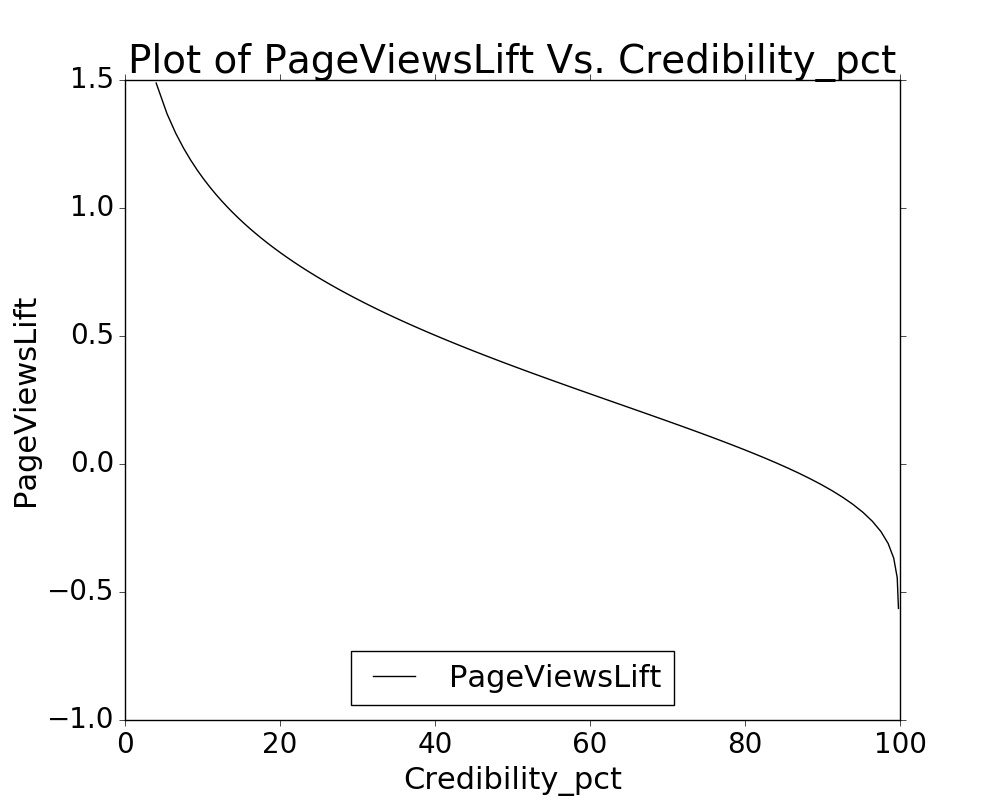
\includegraphics[width=90mm]{figures/PageViewsLift}
\caption{Page Views Lift vs. credibility \label{fig:pv_vs_cred}}
\end{figure}
which as expected is sigmoidal. Thus, we use the data to infer not
just {\em which treatment is better}, but in addition {\em by how
  much} and {\em how certain we are of this}.  In the conventional
approach, we would base our recommendation on a decision criterion
like ``Page Views Lift of 8\% at 95\%
credibility'', and if the point \((95, 0.08)\) is below and to the left of the
above credibility curve in Figure~\ref{fig:pv_vs_cred} we would recommend A over B.

However, from the
perspective of an {\em expected} business return, this process is
ambiguous. Specifically, the above decision point lies above the curve
and so ``A is not better than B''. But the decsiion point also
corresponds to an expected return of \(0.08*0.95 = 0.075\), which is
equivalent to a ``Page Views Lift of 10\% at 75\%
credibility'', which {\em does} lie below the credibility curve and thus
implies a recommendation of ``A is better than B''.
This still does not help either us or the HiPPO, who furthermore
wants to express her or his decision criterion as a single value of expected
return.

Our approach to resolving this conundrum is to interpret
\(M*Cred(M) \) as the {\em expected minimum value} of
\(M\). We plot this as a function of the credibility in
Figure~\ref{fig:exp_pv_vs_cred}.
\begin{figure}[ht!]
\centering
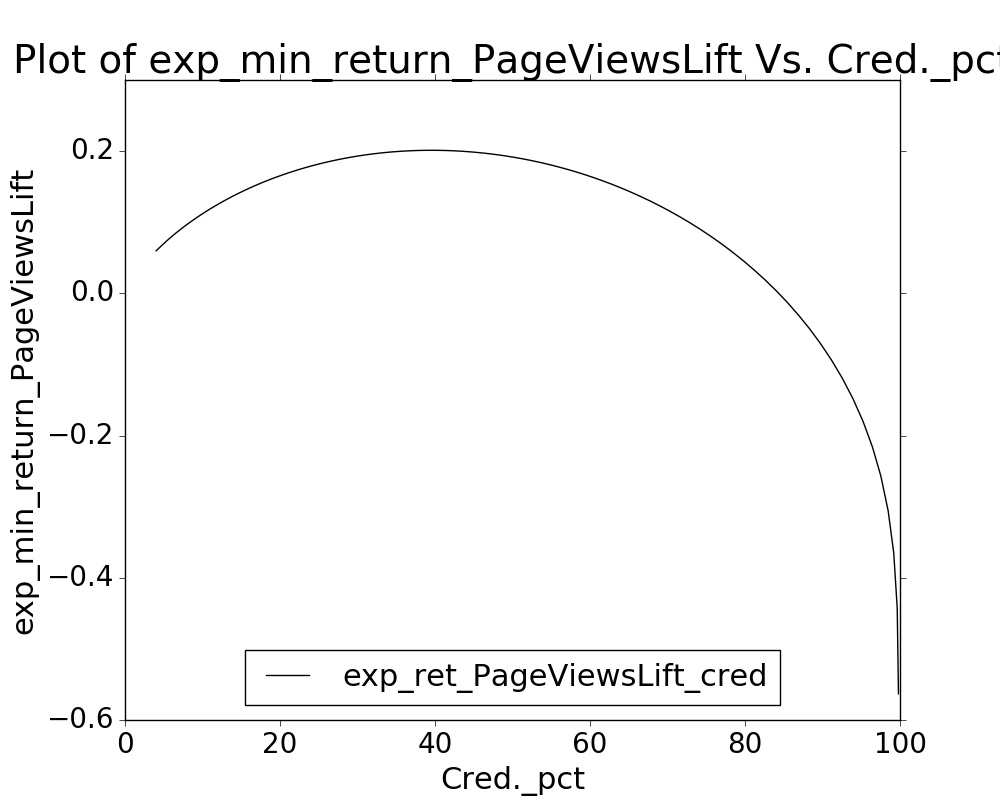
\includegraphics[width=90mm]{figures/exp_ret_PageViewsLift_cred}
\caption{Expected Minimum Page Views Lift vs. Credibility \label{fig:exp_pv_vs_cred}}
\end{figure}
This expected minimum value has a maximum. The question of what recommendation to make is then
reduced to comparing the experimentally determined {\em maximum
  expected minimum value} to the test owner's single value \(M_{Min}\) for an expected return: if the
{\em max-min} is lower than the \(M_{Min}\) then the variant is
{\em not} better than the control. Conversely,
\bdm
    \text{If Max(Expected Minimum} M) > M_{Min}, \text{ then\quad we\quad recommend\quad A\quad over\quad B.}
\edm

Let's recapitulate this last part. The test owner has selected a
metric (let's say Page Views Lift) and a threshold value \(M_{Min}\)
by which A has to exceed B in order for the results to be called in
favor of A. From the data, for every value of the metric \(M\) we can
calculate the credibility (Fig.~\ref{fig:pv_vs_cred}). Note that
\(Cred(M)\) is the credibility that the {\em minimum} true value of
the metric is \(M\). We multiplied \(M\) by its credibility, this is
the {\em expected minimum} value of the metric. As a function of the
credibility (Fig.~\ref{fig:exp_pv_vs_cred}), this expected minimum
itself has a {\em maximum}.  Clearly, if the {\em maximum expected
  minimum value} is less than the minimum acceptable value
\(M_{Min}\), we {\em cannot} call the results in favor of A. If the
opposite holds, we {\em choose} to call the results in favor of A.

To summarize, we've shown two reasons to go beyond the ``Is A better
than B?'' approach to AB testing: One, we have to take the importance
of the difference between A and B into account, and two, we have to
quantify the difference in terms of a business goal. Further, our
approach allows the test owner to establish a single metric and value
as a decision criterion, then our analysis provides a simple ``A/B''
recommendation, without any ``confidence levels'' clouding the issue.


\end{document}

